\documentclass[conference,10pt]{IEEEtran}
\usepackage{amsmath, amssymb}
\usepackage{graphicx}
\usepackage{booktabs}
\usepackage{array}
\usepackage{xcolor}
\usepackage{hyperref}
\hypersetup{colorlinks=true, linkcolor=black, urlcolor=blue!60!black}
\graphicspath{{figures/}}
% table rows generated by make_tables.py; the TeX primitive input can start a table cell, LaTeX's \input cannot
\makeatletter\newcommand{\inputrows}[1]{\@@input #1 }\makeatother

\begin{document}

\title{Mapping a Decade of Research at\\IIT Kharagpur and IIT Roorkee (2016-2026)\\[4pt]
\large Assignment 2, Dynamical Processes in Complex Networks}

\author{\IEEEauthorblockN{Team 3\\Aviral Gupta (2023111023), Varun Shastry (2023112005), Arihant Tripathy (2023111026)}
\IEEEauthorblockA{Dashboard at \url{https://avi1o1.github.io/DPCN_A2_ResearchMapper/}}}

\maketitle

\begin{abstract}
We collected the science and engineering papers of IIT Kharagpur and IIT Roorkee from 2016 to 2026 and linked them to
1,410 faculty members. We study them at the institution, department and faculty level, and we build a citation network
and a co-authorship network. Both IITs almost doubled their output, and most of their journal papers are in Q1 journals.
Their faculty h-index is about half of a career h-index, because we count only ten years of papers. Citations are
heavy-tailed and grow by preferential attachment, but 88\% of the citations inside an institute are self-citations, so
we also rank papers without them. Faculty work in tight, hierarchical groups inside their own IIT. The collaboration
network is a small world that grew denser every year, and it splits into its two campuses when about 100 bridging
faculty are removed.
\end{abstract}

%===========================================================
\section{Introduction}
%===========================================================
Throughout this course, we've looked at how networks can describe real systems, and how measures like centrality and
communities tell us about their structure. In this assignment, we use these ideas on the research of two IITs, IIT
Kharagpur and IIT Roorkee, over the last ten years. We look at this research at three levels, the
\textbf{institution}, its \textbf{departments} and its \textbf{faculty}. Simple counts of papers and citations describe
each of these levels well, but they do not tell us how the research is \textit{connected}. For that, we need networks.
A \textbf{citation network} lets us see how ideas move from one paper to another, while a \textbf{co-authorship
network} lets us see which people actually work together.

We first look at the numbers for each institute as a whole, and then move down to its departments and faculty. Once we
have this picture, we build the two networks and study them, and finally we see how both IITs connect with other
institutes across India. The main numbers of our dataset are summarised in Table~\ref{tab:glance}.

\begin{table}[!h]
\centering
\caption{The dataset at a glance}
\label{tab:glance}
\footnotesize
\setlength{\tabcolsep}{4pt}
\begin{tabular}{@{}lrr@{}}
\toprule
 & \textbf{IIT Kharagpur} & \textbf{IIT Roorkee} \\
\midrule
Papers, 2016-2026                 & 25,950 & 20,326 \\
Papers in 2016 $\rightarrow$ 2025  & 1,583 $\rightarrow$ 2,914 & 1,186 $\rightarrow$ 2,575 \\
Journal papers                     & 19,003 & 14,966 \\
Q1 share of ranked journal papers  & 66.0\% & 60.7\% \\
Journal papers with IF $>$ 5       & 36.0\% & 34.1\% \\
CORE A* / A conference papers      & 98 / 80 & 11 / 34 \\
Faculty with at least one paper    & 770 & 640 \\
Faculty h-index, mean $\pm$ SD (median) & 9.6 $\pm$ 8.6 (8) & 8.7 $\pm$ 7.6 (7) \\
\bottomrule
\end{tabular}
\end{table}

\subsection{Key findings}
\begin{enumerate}
\item From 2016 to 2025, the science and engineering output grew 1.8 times at KGP and 2.2 times at Roorkee, and most of
their ranked journal papers are in Q1 (66.0\% at KGP and 60.7\% at Roorkee).
\item High-IF work comes from small teams. Of the 1,148 KGP and 797 Roorkee papers in journals with IF $>$ 10, 92\%
have fewer than 10 authors (Section~\ref{sec:grid}).
\item 88.5\% of the citations between papers of our two IITs are self-citations, and at equal past citations a
self-citation does not signal later impact the way an outside citation does.
\item Faculty work in tight groups inside their own campus. The two IITs share only 77 direct faculty links, and removing
one faculty member, Dr.~Pradip K.\ Maji, lowers our campus communicability ratio by 31\%.
\item Big teams distort the pair view of collaboration. In our co-authorship data, the papers with more than 10 authors
are 1.8\% of the papers, but they give 27\% of the author pairs, counted paper by paper.
\item Rankings that use the whole network at once, on pairs or on hypergraphs, settle on one dense KGP lab. On the
hypergraph, removing the papers with more than 10 authors changes 17 of the top 20 faculty, while a simple count of
co-authors keeps 16 of its top 20.
\item Trios form along existing pairs. Three authors who have all worked in pairs later write together 3.7\% of the
time, against about 3 in a billion for three people with no joint papers, and 80\% of new trios follow at least one
earlier pair.
\item The collaboration network grew denser every year and survives the random loss of faculty, but removing about 100
bridging faculty splits the two campuses.
\item Faculty cite their co-authors 10 times as often as similar faculty who are far apart, even when the two papers
share no author, and citing and co-authoring each predict the other (Section~\ref{sec:coauthcite}).
\item Teams that mix departments get no citation gain once team size is fixed, but departments do move into research
areas related to what they already do (ROC AUC 0.83 against 0.51 for shuffled areas).
\end{enumerate}

%===========================================================
\section{Data and Methodology}\label{sec:data}
%===========================================================
\textbf{Collecting the papers.} We scraped publication records from public sources like Crossref, Europe PMC, DOAJ, INSPIRE, ORCID, DBLP and Semantic Scholar. We searched in two ways. The first way uses the institute name in the
author affiliations. The second way uses the faculty list of each IIT. This gave 33,393 records for KGP and 25,775
records for Roorkee.

\textbf{Filling in missing values.} A lot of the scraped records had fields missing, so we filled them in using
OpenAlex. This gave us the DOI, type, venue, ISSN, citations, references, author affiliations and the research topic
of each paper. For journal quality, we matched each journal to its \textbf{Scimago} quartile using the ISSN and the
year of publication, and for conferences we used the \textbf{CORE} rank. Later on, we went back to OpenAlex for the yearly citation counts of each paper, the impact factor of each journal, and the career profile of
each faculty member. It is important to note that we did not guess any value. If something could not be found, we
simply left it blank.

\textbf{Checking affiliations.} We kept a paper only if the IIT is in the author affiliations on the paper. This removes namesakes and papers from before a person joined the IIT.

\textbf{Scope.} We keep only \textbf{science and engineering}, as the professor asked. A paper is kept if its OpenAlex topic is in the Physical Sciences or Life Sciences. Health Sciences and Social Sciences papers are left out. We also leave out the faculty of humanities, management, law, education and medical units (for example HSS, the Vinod Gupta School of Management, the School of Medical Science and Technology and the B C Roy hospital). Their science papers stay though, and thus count for the institute. This scope removed 4,069 papers at KGP and 2,518 at Roorkee. We are left with
\textbf{25,950} papers for KGP and \textbf{20,326} for Roorkee.

\textbf{Linking papers to faculty.} The handout asks for one row per paper and faculty member. To link them, we used five rules in order of reliability, the ORCID, the faculty profile we found the paper through, the exact name, the name with the department, and finally the OpenAlex author ID. A few extra checks stop wrong matches, like two faculty sharing a common surname. In the end, 82.8\% of KGP papers and 84.4\% of Roorkee papers have at least one faculty member, and the rest are credited to the institute.

\textbf{Deliverables.} The four files have 54,826 rows (\texttt{group3\_data}), 489,869 citation edges, 137,473
author pairs and 5,367 Indian partners. \texttt{group3\_data} also has the number of authors of each paper and a flag
for papers with more than 10 authors.

\textbf{Note.} 2026 is a \textbf{partial year}, and the citation counts are from October 2026. The h-index and
i10-index use only the 2016-2026 papers in our dataset (Section~\ref{sec:hlow} shows what this means).

%===========================================================
\section{Institution-Level Statistics}\label{sec:inst}
%===========================================================
\subsection{Publication trend}
The simplest measure of research activity is the number of papers per year. We look at it first because it
sets the scale for all other results. More papers give more citations and larger networks. Thus we must keep the size
of each IIT in mind when we compare them.

Both IITs grew steadily (Fig.~\ref{fig:trend}). KGP went from 1,583 papers in 2016 to 2,914 in 2025, which is
\textbf{1.8 times} more. Its peak was 3,094 papers in 2024. Roorkee went from 1,186 papers to 2,575, which is
\textbf{2.2 times} more. KGP is larger every year, but Roorkee grows faster. Not all paper types grew at the same rate.
For KGP, conference papers grew 2.4 times and journal papers grew 1.6 times. For Roorkee the values are 2.9 and 1.9.
Preprints went from almost zero to 130 to 200 each year. So the growth is not only about how much the IITs publish,
but also about \textit{how} they publish. The 2026 bars are low simply because we only have data for a few months.

\begin{figure}[!t]
\centering
\includegraphics[width=0.95\linewidth]{trend.png}
\caption{Papers per year. The faded bars are 2026, which is a partial year.}
\label{fig:trend}
\end{figure}

\subsection{Journal quality}
Counting papers tells us nothing about their quality. For this, we use the Scimago quartile, which ranks the journals of each subject by their SJR score and splits them into four equal parts, with Q1 being the top 25\%. Since journals are ranked \textit{within} their own subject, the Q1 share lets us compare fields that cite at very different rates.

About 95\% of the journal papers of both IITs have a quartile. Of these, 66.0\% at KGP and 60.7\% at Roorkee are in Q1
(Fig.~\ref{fig:quart}), between 27\% and 30\% are in Q2, and only about 1\% are in Q4. This is what we would expect from two of the oldest IITs, which mostly publish in well established journals.

\begin{figure}[!t]
\centering
\includegraphics[width=0.9\linewidth]{quartiles.png}
\caption{Journal quartile mix (Scimago, year of publication).}
\label{fig:quart}
\end{figure}

\subsection{Impact factor}
While the quartile only places a journal in one of four bands, the impact factor (IF) gives us the number of citations a journal gets in a year to its papers from the two years before, divided by the number of
those papers. Clarivate's official Journal Impact Factor is not free, so we apply the same formula to OpenAlex data,
which OpenAlex calls the \textit{2-year mean citedness}. It differs from the official IF in two ways. It is the current value, not the one from the year of publication, and it usually runs higher since OpenAlex counts more citing sources. For example, Scientific Reports has 5.2 here but about 3.8 in Clarivate, so the thresholds below are on the OpenAlex
scale.

The median journal paper sits in a journal with an IF of 4.1 at KGP and 4.0 at Roorkee. 36.0\% of KGP journal papers
and 34.1\% of Roorkee journal papers are in journals with IF $>$ 5, and 6.1\% and 5.3\% are in journals with IF $>$ 10
(1,148 and 797 papers). The share above 5 rose a little over the decade, from about 30\% in 2017-2019 to between 36\%
and 39\% since 2021 (Fig.~\ref{fig:if}). This agrees with the Q1 share above, with KGP slightly ahead on both.

\begin{figure}[!t]
\centering
\includegraphics[width=0.95\linewidth]{impact_factor_over5.png}
\caption{Share of journal papers in journals with IF (OpenAlex) above 5, per year.}
\label{fig:if}
\end{figure}

\subsection{Top journals and important journals}
Table~\ref{tab:journals} shows the top 10 journals of each IIT with their IF. All are Q1, except ChemistrySelect (Q2).
Some are broad journals, such as Scientific Reports and RSC Advances. Others match a strong area of each IIT, such as fluid mechanics at KGP (Physics of Fluids) and nuclear physics at Roorkee (Physical Review C).

\begin{table}[!t]
\centering
\caption{Top 10 journals of each IIT by papers, with IF (OpenAlex)}
\label{tab:journals}
\footnotesize
\begin{tabular}{@{}lrr@{}}
\toprule
\textbf{Journal} & \textbf{Papers} & \textbf{IF} \\
\midrule
\multicolumn{3}{@{}l}{\emph{IIT Kharagpur}} \\
Physics of Fluids & 325 & 4.2 \\
Scientific Reports & 175 & 5.2 \\
ACS Applied Materials \& Interfaces & 149 & 8.8 \\
Langmuir & 130 & 4.9 \\
RSC Advances & 112 & 7.5 \\
Physical Chemistry Chemical Physics & 107 & 3.6 \\
Journal of Alloys and Compounds & 96 & 6.3 \\
ACS Applied Nano Materials & 95 & 6.9 \\
Science of The Total Environment & 93 & 12.2 \\
Materials Science and Engineering A & 88 & 6.8 \\
\midrule
\multicolumn{3}{@{}l}{\emph{IIT Roorkee}} \\
Scientific Reports & 124 & 5.2 \\
Int.\ J.\ of Biological Macromolecules & 120 & 9.2 \\
Physical Review C & 117 & 3.2 \\
IEEE Trans.\ on Industry Applications & 110 & 4.4 \\
Environ.\ Science and Pollution Research & 101 & 6.4 \\
Physics of Fluids & 86 & 4.2 \\
IEEE Access & 85 & 6.4 \\
ChemistrySelect & 78 & 2.5 \\
IEEE Trans.\ on Electron Devices & 77 & 3.6 \\
J.\ of Environmental Chemical Engineering & 70 & 6.1 \\
\bottomrule
\end{tabular}
\end{table}

Some journal groups are seen as important in physics and chemistry. These are the American Physical Society
(APS) journals (the Physical Review family), Physical Review Letters (PRL), the SPIE journals, the Nature journals and
the Journal of the American Chemical Society (JACS). Counting these papers shows how often the IITs publish at the top
of these fields. The counts are in Table~\ref{tab:important}. The APS journals are the largest group, with about 300
papers at KGP and 230 at Roorkee. At KGP they are spread over Physical Review A, B, D and E, and at Roorkee half of
them are in Physical Review C (nuclear physics). Papers in PRL, Nature journals and JACS
are rare, with 6 to 25 papers each over ten years. This is expected, because these journals accept very few papers.

\begin{table}[!t]
\centering
\caption{Papers in important journal groups, 2016-2026}
\label{tab:important}
\footnotesize
\begin{tabular}{@{}lrr@{}}
\toprule
\textbf{Group} & \textbf{KGP} & \textbf{Roorkee} \\
\midrule
APS (all Physical Review journals) & 299 & 231 \\
\quad of which PRL & 10 & 6 \\
SPIE journals & 17 & 22 \\
SPIE conference proceedings & 8 & 8 \\
Nature journals (Nature, Nature Communications, ...) & 25 & 22 \\
JACS & 9 & 14 \\
\bottomrule
\end{tabular}
\end{table}

\subsection{PRL and the Nature journals}
We now look at the two smallest groups in more detail. Table~\ref{tab:prl} lists all 16 PRL papers, 10 from KGP and 6
from Roorkee. The KGP papers have small teams of 3 to 13 authors, while four of the six Roorkee papers come from
nuclear and particle physics, where teams of 20 or more are normal. One KGP entry is a reply to a comment, and not a
research paper. The most cited one is the 2017 KGP paper on the planar Hall effect in Weyl semimetals (351 citations).
PRL has an IF of 9.05 on our OpenAlex scale, so it falls just below the IF $>$ 10 band used later.

\begin{table*}[!t]
\centering
\caption{All papers in Physical Review Letters, 2016-2026 (``(institute)'' means no faculty member could be linked)}
\label{tab:prl}
\footnotesize
\begin{tabular}{@{}llp{9.0cm}p{3.6cm}rr@{}}
\toprule
 & \textbf{Year} & \textbf{Title} & \textbf{Faculty} & \textbf{Auth.} & \textbf{Cit.} \\
\midrule
\inputrows{tables/prl.tex}
\end{tabular}
\end{table*}

Our papers appear in 16 Nature journals (Table~\ref{tab:nature}). All of them have an IF above 10, except Nature Cities
(9.3). Nature Communications has more than half of the 47 papers, with 12 from KGP and 13 from Roorkee.

\begin{table}[!t]
\centering
\caption{Nature journals in our data, with IF (OpenAlex) and papers}
\label{tab:nature}
\footnotesize
\begin{tabular}{@{}lrrr@{}}
\toprule
\textbf{Journal} & \textbf{IF} & \textbf{KGP} & \textbf{Roorkee} \\
\midrule
\inputrows{tables/nature.tex}
\end{tabular}
\end{table}

\subsection{Conferences and CORE}
For conference papers we use the \textbf{CORE} rank (A*, A, B, C). CORE ranks mostly computing conferences. Thus it
tells us about the computer science side of each IIT, and most conference papers have no CORE rank.

At KGP, 522 of 3,814 conference papers (13.7\%) are in CORE-ranked venues. These are 98 A*, 80 A, 222 B and 122 C
papers. At Roorkee, 289 of 3,211 (9.0\%) are ranked. These are 11 A*, 34 A, 144 B and 100 C papers. Thus KGP is far
ahead at the top ranks. Computer Science is 14.1\% of KGP papers and only 8.9\% of Roorkee
papers. The most frequent CORE venue is the same for both IITs. It is the IEEE Geoscience and Remote Sensing
Symposium (rank C, 51 KGP papers and 81 Roorkee papers). The KGP list also has top venues such as AAAI (A*, 16
papers) and CIKM (A, 17 papers). Ranked conference papers increased after 2021 at both IITs.

\subsection{Research areas and their categories}
Next, we look at what each IIT works on. OpenAlex places every paper in a four-level hierarchy, the
\textit{domain}, \textit{field}, \textit{subfield} and \textit{topic}. For example, a paper on perovskite solar cells falls under the domain Physical Sciences, the field Engineering, the subfield Electrical and Electronic Engineering, and the topic Perovskite Materials and Applications. These research areas matter for the rest of the report too, since they decide which papers can cite each other and which faculty can work together.

\textbf{Engineering} is the largest field at both IITs, with 36.6\% of KGP papers and 43.3\% of Roorkee papers
(Fig.~\ref{fig:areas}). Inside Engineering the main subfields are Electrical and Electronic Engineering (24\% at KGP
and 32\% at Roorkee), Mechanical Engineering, Biomedical Engineering and Civil and Structural Engineering. After
Engineering, KGP has more Computer Science (14.1\%) and Roorkee has more Environmental Science (12.7\%). Materials
Science is about 11\% at both. The dashboard lists the subfields inside every field.

\begin{figure}[!t]
\centering
\includegraphics[width=0.95\linewidth]{research_areas.png}
\caption{Share of papers by OpenAlex field (primary topic).}
\label{fig:areas}
\end{figure}

\textbf{Why is Environmental Science so high?} It is 10.4\% of KGP papers and 12.7\% of Roorkee papers. The subfields explain it (Fig.~\ref{fig:env}). About two thirds of these papers are in Environmental Engineering, Water Science and Technology, and Global and Planetary Change. The most common topics are hydrology, watershed management, floods, climate models and the removal of pollutants from water. The departments of the authors are mostly engineering departments. At KGP these are Civil Engineering (28\% of these papers), Agricultural and Food Engineering and the CORAL centre. At Roorkee they are Civil Engineering (21\%), Hydrology and Water Resources Development and Management. Thus Environmental Science is high, because OpenAlex puts much of the water and climate engineering of the two IITs in this field. Roorkee has entire departments for hydrology and water resources, so its share is higher.

\begin{figure}[!t]
\centering
\includegraphics[width=0.95\linewidth]{env_science_subfields.png}
\caption{Subfields inside Environmental Science.}
\label{fig:env}
\end{figure}

\subsection{Most-cited papers and large collaborations}
The last measure at this level is the number of worldwide citations of each paper. The most cited papers are the most visible work of each IIT, but some of them say more about the \textit{type} of paper than about the institute itself.

Table~\ref{tab:cited} shows the top three papers of each IIT. At KGP, two of them are software tools (SymPy and
iFogSim). At Roorkee, the top paper is a large collaboration (the European Pulsar Timing Array), and at least five of the top ten are reviews or surveys. This makes sense, since anyone working on a topic or using a tool ends up citing its review or tool paper, so such papers collect citations very quickly.

\begin{table}[!t]
\centering
\caption{Most-cited papers (worldwide, October 2026)}
\label{tab:cited}
\footnotesize
\begin{tabular}{@{}l>{\raggedright\arraybackslash}p{5.0cm}r@{}}
\toprule
 & \textbf{Paper (year)} & \textbf{Cit.} \\
\midrule
KGP & Soil carbon 4 per mille (2017) & 2,020 \\
KGP & SymPy, symbolic computing in Python (2017) & 1,502 \\
KGP & iFogSim, a toolkit for modeling and simulation of resource management techniques ... (2017) & 1,250 \\
\midrule
Roork. & The second data release from the European Pulsar Timing Array (2023) & 1,069 \\
Roork. & A comprehensive review on NSGA-II for multi-objective combinatorial optimization (2021) & 971 \\
Roork. & Microwave--material interaction phenomena, heating mechanisms ... (2016) & 876 \\
\bottomrule
\end{tabular}
\end{table}

We \textbf{flag papers with more than 10 authors}, because in such papers our faculty are one group among many. They are few, 534 papers at KGP (2.1\%) and 454 at Roorkee (2.2\%). 17 and 7 of them have 100 or more authors. But they get more than their share of citations, 6.0\% of all KGP citations and 3.7\% of all Roorkee citations. The flag is in \texttt{group3\_data.csv} and on the dashboard.

\subsection{How much do large collaborations matter?}
To see how much our numbers depend on these papers, we recomputed every headline number without them
(Fig.~\ref{fig:large}, left). The \textit{typical} paper barely changes. The median paper still has 6 citations at KGP
and 5 at Roorkee, and the Q1 share drops by only half a point. The \textit{top}, however, does change. At KGP, 6 of the
10 most cited papers have more than 10 authors (2 at Roorkee). Without them, KGP loses 9.3\% of its papers with 100 or
more citations, and its institute h-index falls from 184 to 176, while Roorkee's falls from 156 to 154. The faculty
h-index moves too, with 74 KGP faculty (9.6\%) and 57 Roorkee faculty (8.9\%) losing at least one point, and the median
KGP faculty h-index dropping from 8 to 7.

\textbf{A citation premium.} Large papers get more citations than other papers from the same IIT and year
(Fig.~\ref{fig:large}, right). At KGP, the median large paper gets 2.7 times the citations of the median other paper
(median over 2016-2024), while at Roorkee the premium is smaller, at 1.25 times. One reason is simply that more
authors means more people citing the paper, and more networks that come across it.

\textbf{What these papers are.} 82\% of the large journal papers at KGP are in Q1 journals, against 62\% for its other
papers (Roorkee 76\% against 57\%). Only 2-3\% are conference papers, against 15-16\% of the other papers, and 81\%
have a co-author abroad (Roorkee 76\%), against 22-23\% of the rest. So large teams mostly mean international
collaboration. Most of them are not huge either, as 86\% of the KGP and 76\% of the Roorkee large papers have 11 to 20
authors, and only 17 and 7 papers have 100 or more.

\textbf{Where they come from.} At KGP, they mostly come from materials research, with Metallurgical and Materials
Engineering (78 papers), Physics (60), Agricultural and Food Engineering (60) and Biosciences (45). Materials Science is
the largest field (22\% of them), and the top venues are \textit{Small}, \textit{Advanced Functional Materials} and
\textit{ACS Applied Materials \& Interfaces}. At Roorkee, they come mostly from Physics (134 papers, 30\% of Roorkee's
large papers and 9\% of its physics papers), followed by Biosciences (74) and Hydrology (28). The top venue here is
\textit{Physical Review C} (44 papers) from nuclear physics collaborations, and the pulsar timing papers show up too.

\textbf{Who depends on them.} For a few faculty, large papers make up a big part of their h-index. At KGP, the h-index
of Dr. Tapas Kumar Maiti (Biosciences) falls from 36 to 30 without them, and that of Dr. Abhijit Mukherjee (Geology and
Geophysics) from 44 to 39. At Roorkee, the largest drop is in Physics, where Dr. Bhal Chandra Joshi, who works on pulsar timing arrays, goes from 8 to 2. This does not make these papers any less valuable. But an h-index built on large
collaborations measures something different from one built in a small group, which is why we show both on the
dashboard.

\begin{figure*}[!t]
\centering
\includegraphics[width=0.85\linewidth]{large_collab_effect.png}
\caption{Papers with more than 10 authors, with the change in the headline numbers without them (left), and their
median citations divided by the median of the institute's other papers from the same year (right).}
\label{fig:large}
\end{figure*}

\subsection{High-IF papers and team size}\label{sec:grid}
A paper with a few authors says more about the group itself than a paper with a hundred. So we split the best journal
papers by team size in Table~\ref{tab:grid}. The rows get stricter, from Q1, to Q1 with IF $>$ 5, to Q1 with IF $>$ 10.
We give exactly 10 authors its own column, so that every row adds up. These counts are for Q1 and high-IF journal
papers only, so they are a part of the 534 and 454 large papers above.

At both IITs, more than 90\% of the papers in every row have fewer than 10 authors. Large teams do become a little more
common as the bar rises. At KGP, 3.3\% of the Q1 papers have more than 10 authors, against 6.3\% of the Q1 papers with
IF $>$ 10 (Roorkee 3.5\% and 5.2\%). This fits what we saw above, as large papers are more often in Q1 journals. Almost
every paper with IF $>$ 10 is also Q1 (1,119 of 1,148 at KGP and 783 of 797 at Roorkee).

So the high-IF output of both IITs comes from small teams, with 1,057 papers at KGP and 736 at Roorkee. They are spread
over 152 and 110 journals. The five most common journals of each IIT are in Table~\ref{tab:if10j}. They are mostly
environmental, chemical engineering and construction journals, which matches the strength in Environmental Science that
we saw in the research areas.

\begin{table}[!t]
\centering
\caption{Journal papers by quality and number of authors (journal papers only)}
\label{tab:grid}
\footnotesize
\setlength{\tabcolsep}{3pt}
\begin{tabular}{@{}lrrrrr@{}}
\toprule
 & \textbf{Papers} & \textbf{$<$10} & \textbf{10} & \textbf{$>$10} & \textbf{$>$10 share} \\
\midrule
\inputrows{tables/if_grid.tex}
\end{tabular}
\end{table}

\begin{table}[!t]
\centering
\caption{Most common journals of the IF $>$ 10 papers with fewer than 10 authors}
\label{tab:if10j}
\footnotesize
\begin{tabular}{@{}lrr@{}}
\toprule
\textbf{Journal} & \textbf{IF} & \textbf{Papers} \\
\midrule
\inputrows{tables/if10_journals.tex}
\end{tabular}
\end{table}

%===========================================================
\section{Faculty and Department Level}\label{sec:fac}
%===========================================================
Everything so far is really a sum over people. So we now look at the faculty themselves, and then at the departments
they belong to.

\subsection{h-index statistics}
A faculty member has an \textbf{h-index} of $h$ if $h$ of their papers have at least $h$ citations each. This measure
combines how much a person publishes and how much other people cite it. One very large paper cannot increase it alone.

The h-index is strongly right-skewed (Fig.~\ref{fig:h}). Many faculty have a small h-index, and a few have a very large
one. Thus the mean alone is misleading, and we give several statistics (Table~\ref{tab:hstats}). At KGP the mean is
9.6 with a standard deviation of 8.6, and the median is 8. At Roorkee the mean is 8.7 with a standard deviation of 7.6,
and the median is 7. The SD is almost as large as the mean, which again shows the long tail. The highest values are 63
at KGP (Dr.~Narayan Chandra Das, Rubber Technology) and 53 (Dr.~Makarand M.\ Ghangrekar, Civil Engineering), and 42 at
Roorkee (Dr.~Soumitra Satapathi, Physics).

\begin{table}[!t]
\centering
\caption{Faculty h-index and i10-index (2016-2026 papers)}
\label{tab:hstats}
\footnotesize
\setlength{\tabcolsep}{3pt}
\begin{tabular}{@{}lrrrr@{}}
\toprule
 & \multicolumn{2}{c}{\textbf{h-index}} & \multicolumn{2}{c}{\textbf{i10-index}} \\
 & \textbf{KGP} & \textbf{Roorkee} & \textbf{KGP} & \textbf{Roorkee} \\
\midrule
Faculty & 770 & 640 & 770 & 640 \\
Mean $\pm$ SD & 9.6 $\pm$ 8.6 & 8.7 $\pm$ 7.6 & 13.9 $\pm$ 21.7 & 11.6 $\pm$ 17.2 \\
Median & 8 & 7 & 6 & 5 \\
Middle half (Q1--Q3) & 3--13 & 3--12 & 1--16 & 1--14 \\
90th percentile & 22 & 19 & 37 & 30 \\
Maximum & 63 & 42 & 184 & 122 \\
\bottomrule
\end{tabular}
\end{table}

\begin{figure}[!t]
\centering
\includegraphics[width=0.95\linewidth]{h_index_hist.png}
\caption{Distribution of the faculty h-index (2016--2026 papers in our dataset).}
\label{fig:h}
\end{figure}

\subsection{i10-index}
The i10-index is the number of papers with at least 10 citations. It is used by Google Scholar. It is simpler
than the h-index, and it shows how many of a person's papers are cited well. The median faculty member has 6 such papers at KGP and 5 at Roorkee in these ten years. The mean is much higher (13.9 and 11.6), because a few very active labs have more than 100 such papers each (Table~\ref{tab:hstats}).

\subsection{Why is the computed h-index low?}\label{sec:hlow}
A median h-index of 7 or 8 seems low for faculty at two of the oldest IITs, so we looked into why. For each faculty
member, we compare three values, the h-index we computed, the h-index of the same papers using OpenAlex citation counts
instead, and the h-index of their whole OpenAlex profile, which covers their entire career. We only use the career
value when the profile clearly belongs to that person (at least 5 of their papers checked, with at least 80\% of them on that profile), since some profiles merge two people with the same name. This leaves 565 faculty at KGP and 437 at Roorkee.

\begin{table}[!t]
\centering
\caption{Median faculty h-index, three ways}
\label{tab:hcheck}
\footnotesize
\begin{tabular}{@{}lrr@{}}
\toprule
 & \textbf{KGP} & \textbf{Roorkee} \\
\midrule
Our h-index (2016--2026 papers) & 9 & 9 \\
Same papers, OpenAlex citation counts & 10 & 9 \\
OpenAlex profile, whole career & 20 & 19 \\
\bottomrule
\end{tabular}
\end{table}

Table~\ref{tab:hcheck} gives the answer. The citation source barely matters, as the same papers give almost the same
h-index with OpenAlex counts. The real difference is the \textit{time window}. The computed h-index only counts papers
from 2016 to 2026, while a career h-index also counts all the older papers, which have had many more years to collect
citations. So the computed value is about half of the career value (53\% at KGP and 50\% at Roorkee at the median), and
98\% of faculty are below their career value (Fig.~\ref{fig:hcheck}). Google Scholar is higher still, since it also
counts preprints, theses and books. For example, Dr.~A.\ Taraphder's 2017 PRL paper has 351 citations in our data and
435 on Google Scholar, and the paper is in our dataset, linked to him by his ORCID.

\begin{figure}[!t]
\centering
\includegraphics[width=0.95\linewidth]{h_index_check.png}
\caption{The computed h-index against the OpenAlex whole-career h-index (the dashed line marks equal values).}
\label{fig:hcheck}
\end{figure}

\subsection{h-index over the years}
The h-index grows with time, because a person writes more papers and the old papers collect citations. To see this
growth, we compute the h-index at the end of each year. For year $Y$ we use the papers published up to $Y$ and only the
citations received up to $Y$, from the yearly citation counts in OpenAlex.

The mean faculty h-index rose from 0.9 at the end of 2016 to 9.5 at the end of 2025 at KGP, and from 0.8 to 8.5 at
Roorkee (Fig.~\ref{fig:hyear}). It grows by about one point each year at both IITs, and KGP stays a little ahead. The
h-index of each institute as a whole, computed over all its papers, grew from 10 to 178 at KGP and from 12 to 153 at
Roorkee. The growth is steady. This agrees with the growing output and the growing citations
from Indian institutes (Section~\ref{sec:cit}).

\begin{figure}[!t]
\centering
\includegraphics[width=\linewidth]{h_index_by_year.png}
\caption{h-index at the end of each year. Left, the mean faculty h-index. Right, the h-index of each institute.}
\label{fig:hyear}
\end{figure}

\subsection{Departments}
Departments are between the person and the institute. They are the natural unit to compare research areas inside one
IIT. Table~\ref{tab:dept} shows the five departments with the most papers at each IIT.

At KGP, Computer Science has the most papers, but Civil Engineering has the most citations (41,228). Civil Engineering
includes environmental engineering, and two of the five highest h-index values at KGP are in this department. At
Roorkee, Civil Engineering has the most papers and the most faculty (75). The Q1 share is between 50\% and 73\% in the
engineering departments. Mathematics is much lower at both IITs, at about 45\%. We expect this, because mathematics
journals have lower impact scores in general. The mean h-index of a department is close to its SD, so every department
has a mix of young and very senior faculty.

\begin{table}[!t]
\centering
\caption{Top 5 departments of each IIT by number of papers}
\label{tab:dept}
\footnotesize
\setlength{\tabcolsep}{2.5pt}
\begin{tabular}{@{}lrrrrr@{}}
\toprule
\textbf{Department} & \textbf{Fac.} & \textbf{Papers} & \textbf{Cit.} & \textbf{Q1} & \textbf{h, mean$\pm$SD} \\
\midrule
\multicolumn{6}{@{}l}{\emph{IIT Kharagpur}} \\
Computer Sci.\ \& Engg.    & 51 & 2,429 & 25,758 & 66.9\% & 9.0 $\pm$ 7.9 \\
Mechanical Engg.           & 54 & 1,926 & 29,048 & 71.3\% & 11.0 $\pm$ 9.3 \\
Civil Engg.                & 45 & 1,748 & 41,228 & 70.8\% & 12.7 $\pm$ 10.9 \\
Chemistry                  & 42 & 1,650 & 36,372 & 72.8\% & 14.0 $\pm$ 9.3 \\
Agri.\ \& Food Engg.       & 52 & 1,480 & 32,085 & 61.5\% & 10.8 $\pm$ 8.5 \\
\midrule
\multicolumn{6}{@{}l}{\emph{IIT Roorkee}} \\
Civil Engg.                & 75 & 2,021 & 26,979 & 56.2\% & 8.5 $\pm$ 6.6 \\
Electronics \& Comm.       & 45 & 1,854 & 15,978 & 49.7\% & 7.9 $\pm$ 6.0 \\
Electrical Engg.           & 48 & 1,694 & 16,424 & 68.7\% & 8.3 $\pm$ 6.6 \\
Mech.\ \& Industrial Engg. & 53 & 1,671 & 30,210 & 61.4\% & 11.2 $\pm$ 8.2 \\
Physics                    & 44 & 1,515 & 20,711 & 65.8\% & 9.4 $\pm$ 7.9 \\
\bottomrule
\end{tabular}
\end{table}

%FACULTY-BY-YEAR

%===========================================================
\section{Citation Network}\label{sec:cit}
%===========================================================
So far, every citation has counted the same. A network lets us go one step further and ask \textit{who} cites whom.

\subsection{Construction}
Each node is a paper from one of our two IITs, and a directed edge $A \to B$ means that paper $A$ cites paper $B$,
with both papers in our dataset. The edges are directed because a citation only goes one way, from a newer paper to an
older one. The network has 46,072 papers and 86,090 edges, with 25,942 papers and 47,586 edges for KGP, and 20,326
papers and 35,246 edges for Roorkee. It is also very sparse, with a density of $4.1\times10^{-5}$ and a mean in-degree
of 1.9. About half of the papers are never cited by another paper from the two IITs, and the largest weakly connected
component holds 53\% of the papers. This is what we would expect, since the papers come from many fields that rarely
cite each other.

\subsection{In-degree distribution}
As we saw in the lectures, the in-degree of a node is the number of edges pointing to it. Here, it is the number of
papers in our dataset that cite a given paper. Its distribution tells us whether attention is spread evenly, or goes to
only a few papers.

Fig.~\ref{fig:indeg} shows $P(\text{in-degree} \ge k)$ on a log-log scale. The curve falls slowly over two orders of
magnitude, so the distribution is heavy-tailed. Most papers get zero, one or two internal citations, but a few get 40
to 58. The curves for the two IITs are almost the same, which tells us that the shape comes from how citation works in
general, and not from anything specific to one institute.

\begin{figure}[!t]
\centering
\includegraphics[width=0.6\linewidth]{indegree_ccdf.png}
\caption{In-degree distribution of the citation network (CCDF, log-log).}
\label{fig:indeg}
\end{figure}

\subsection{Is it a power law?}
A straight line on a log-log plot is not enough to call something a power law. So we follow the method of Clauset,
Shalizi and Newman, which fits $P(k) \propto k^{-\alpha}$ above a cut-off $x_{\min}$ by maximum likelihood, and then
compares the power law with other heavy-tailed distributions using a likelihood ratio test (Fig.~\ref{fig:fit}).

For the internal in-degree, the fit gives $\alpha = 2.81$ above $x_{\min}=5$. However, the lognormal fits much better
(normalised ratio $R=-13.3$, $p<0.001$), because the curve bends down at the end. This is not surprising, since a
paper can only get a few dozen citations at most from inside two institutes. For the global citation counts, the tail
above 73 citations (1,861 papers) has $\alpha = 3.00 \pm 0.05$. Here the power law does much better than an
exponential ($R=5.4$, $p<0.001$), but we cannot tell it apart from a lognormal ($p=0.16$). So we can call the
distribution ``heavy-tailed'', but not ``scale-free'', which is also what large studies of citations tend to find.

\begin{figure}[!t]
\centering
\includegraphics[width=\linewidth]{citation_distribution_fit.png}
\caption{Maximum-likelihood fits of the tail, with the power law in grey and the lognormal in orange.}
\label{fig:fit}
\end{figure}

\subsection{Preferential attachment, measured}
In the lectures, the Barab\'asi--Albert model explains heavy tails through preferential attachment, where a node with
degree $k$ gets new links at a rate $\Pi(k) \propto k$. Since our citations are dated, we can actually measure this.
For each year $T$ from 2017 to 2025, we take every paper that already existed, count its citations $k$ up to year
$T-1$, and then count the new citations it got in year $T$. The mean number of new citations at each $k$ gives the
attachment rate $A(k)$. We use both the internal citations and the citations from other Indian institutes here, since
both come with a year.

Fig.~\ref{fig:pa} shows that $A(k)$ grows steadily with $k$, with a paper that has 10 citations getting about three
times as many new citations as one that has a single citation. The best fit is $A(k) = c\,(k + k_0)^{\alpha}$ with
$\alpha = 0.80 \pm 0.02$ and $k_0 = 1.8$, so the attachment is slightly sublinear. The $k_0$ term is the ``initial
attractiveness'', meaning that even an uncited paper still gets 0.57 new citations a year. A sublinear $\alpha$ gives a
stretched-exponential or lognormal shape rather than a pure power law, which agrees with the fits above. One caveat is
that papers also differ in quality (their ``fitness''), and better papers tend to be cited both earlier and later, so
part of the measured effect could come from this.

\begin{figure}[!t]
\centering
\includegraphics[width=0.62\linewidth]{preferential_attachment.png}
\caption{Attachment rate $A(k)$, the new citations in a year for a paper with $k$ earlier citations.}
\label{fig:pa}
\end{figure}

\subsection{Self-citations}
The handout defines the in-degree as the number of citations from the same institute's papers, so we checked where
these citations actually come from. We call an edge a self-citation if the citing and the cited paper share an author
(the same OpenAlex author, or the same faculty member). It turns out that 88.5\% of the 86,090 internal edges are
self-citations (KGP 92.8\%, Roorkee 90.1\%), and only 9,909 edges connect different authors. The share drops from 98\%
in 2016 to 87-89\% in 2026 (Fig.~\ref{fig:self}), simply because over time, there are more papers by colleagues that
one can cite.

This changes how we should read the internal network, since it mostly shows researchers building on \textit{their own}
earlier work. There are 42 papers with zero citations worldwide but five or more internal citations, and all of these
are self-citations. Also, 79\% of the edges stay within one OpenAlex field (field assortativity 0.73), and so do 76\% of
the non-self edges. So ideas rarely move between fields, even between colleagues.

\begin{figure}[!t]
\centering
\includegraphics[width=0.62\linewidth]{self_citation_yearly.png}
\caption{Share of internal citations that are self-citations, by year of the citing paper.}
\label{fig:self}
\end{figure}

\subsection{PageRank}
As covered in class, \textbf{PageRank} scores a node based not only on how many nodes point to it, but also on how
important those nodes are.
\[
PR(i) = \frac{1-\alpha}{N} + \alpha \sum_{j \to i} \frac{PR(j)}{k_{\text{out}}(j)}, \qquad \alpha = 0.85
\]
Here, $N$ is the number of papers and $k_{\text{out}}(j)$ is the number of papers that $j$ cites. While the in-degree
treats every citation the same, PageRank gives more weight to a citation from an influential paper. So it picks out the
papers that other well-cited work is \textit{built on}.

Our data shows this clearly (Table~\ref{tab:pr}). The top paper by PageRank is a 2016 KGP paper on MoS$_2$
heterojunctions, which has only 20 internal citations and an in-degree rank of 195, but the papers citing it are
themselves highly cited. There is also an age bias, as seven of the top ten papers are from 2016, and the Spearman
correlation between PageRank and publication year is $-0.39$. This makes sense, because in a citation network the
score flows almost entirely from newer papers to older ones, so the oldest papers in our window end up with the most.

\begin{table}[!t]
\centering
\caption{Top 5 papers by PageRank (both IITs), with in-degree and in-degree rank}
\label{tab:pr}
\footnotesize
\begin{tabular}{@{}l>{\raggedright\arraybackslash}p{4.4cm}rr@{}}
\toprule
 & \textbf{Paper (year)} & \textbf{In} & \textbf{Rank} \\
\midrule
KGP    & Hydrothermal growth of few layer 2H-MoS$_2$ for heterojunction ... (2016) & 20 & 195 \\
KGP    & Uniform electric-field-induced lateral migration of a sedimenting drop (2016) & 58 & 1 \\
KGP    & V$_2$O$_5$ microflower decorated cathode for enhancing power ... (2016) & 23 & 108 \\
Roork. & A review of power electronic converters for variable speed pumped storage ... (2018) & 49 & 4 \\
KGP    & Groundwater quality and depletion in the Indo-Gangetic Basin ... (2016) & 51 & 2 \\
\bottomrule
\end{tabular}
\end{table}

\subsection{Correcting PageRank}
The two problems we found above, self-citations and age, affect PageRank too, so we made two corrections.

First, we ran PageRank on only the 9,909 non-self edges. Only 7 of the original top 100 papers stay in the top 100, and
the new top papers are the ones cited by other groups, like a review of Himalayan--Karakoram glaciers (Roorkee, 331
citations worldwide) and studies of rainfall and drought over India (KGP). Second, we removed the age bias using the
rescaled PageRank of Mariani, Medo and Zhang, where each paper's score becomes a $z$-score among papers from the same
year, $R_i = (p_i - \mu_{y(i)})/\sigma_{y(i)}$. The test for a fair ranking is simple, as every year should have about
1\% of its papers in the overall top 1\%. Fig.~\ref{fig:agebias} shows the result. With plain PageRank, 6.5\% of the
2016 papers make the top 1\%, but not a single paper from 2024 or 2025 does. The coefficient of variation of these
shares falls from 1.44 (PageRank) to 0.87 (no self-citations), and then to 0.20 (rescaled). In the rescaled top 10,
papers from 2023-2025 show up next to older ones, and these are the papers that started strongly for their age.

\begin{figure}[!t]
\centering
\includegraphics[width=0.62\linewidth]{pagerank_age_bias.png}
\caption{Share of each year's papers in the top 1\% of three rankings (2016-2025 papers).}
\label{fig:agebias}
\end{figure}

\subsection{Citation flow with other Indian institutes}
The network above stays within our two IITs. To see where they stand in Indian research as a whole, we also count
citations to and from other Indian institutes. The in-flow is the number of citations our papers get from papers of
other Indian institutes, and the out-flow is the number of citations our papers give to theirs. The impact ratio is the
in-flow divided by the out-flow, so a ratio above 1 means that Indian research cites the IIT more than the IIT cites
Indian research.

KGP has an in-flow of 102,511 and an out-flow of 115,479, giving a ratio of 0.89, while Roorkee has 86,983 and
107,630, giving 0.81. At first glance, it looks like both IITs give out more citations than they get, but
Fig.~\ref{fig:flow} shows why. In 2016, our papers were already citing thousands of older Indian papers (the KGP
out-flow was 5,335), but almost nobody had cited them yet (the KGP in-flow was 214), since citations take years to
arrive. The in-flow grows much faster over time, and has been larger than the out-flow since 2023 at KGP and since 2024
at Roorkee. So the overall ratio below 1 is mostly a result of the 2016-2026 window.

The largest Indian source of citations to KGP is IIT Roorkee (2,914 citations), followed by VIT and AcSIR, while for
Roorkee it is UPES (2,345), followed by VIT and AcSIR. Large universities like VIT, UPES and Saveetha cite our IITs much
more than our IITs cite them (ratios between 1.6 and 3.7). The most cited Indian paper citing KGP is the SciPy 1.0
paper, and the most cited one citing Roorkee is a paper on drug delivery vehicles for cancer treatment.

\begin{figure}[!t]
\centering
\includegraphics[width=0.92\linewidth]{citation_flow_yearly.png}
\caption{Citation in-flow and out-flow with other Indian institutes, per year.}
\label{fig:flow}
\end{figure}

%===========================================================
\section{Co-authorship Network}\label{sec:auth}
%===========================================================
While the citation network shows how \textit{ideas} move, the co-authorship network shows how \textit{people} work
together, which is much closer to how research groups actually function.

\subsection{Construction}
Each node is a faculty member from one of the two IITs, and an undirected edge connects two faculty who have written at
least one paper together, weighted by the number of joint papers. The network has 1,410 faculty and 2,719 edges, with a
density of 0.0027. On average, a faculty member has 3.9 faculty co-authors, and 254 faculty have none at all. The
largest component, shown in Fig.~\ref{fig:net}, holds 79\% of all faculty. The two IITs form two separate clusters,
with only 77 edges between them, which is natural given that the campuses are far apart and most work happens within
one campus.

The faculty network is only a small slice of all co-authorship, though. A faculty member has a median of 25 distinct
co-authors, and of all the author pairs in \texttt{authorship\_network.csv} involving a faculty member, 52\% are with
students and staff of the same IIT, 21\% with other Indian institutes, 17\% with foreign institutes, and only 7\% with
another faculty member of our two IITs. So the faculty network really shows the links \textit{between} research groups,
while students make up most of each group.

\begin{figure}[!t]
\centering
\includegraphics[width=0.5\linewidth]{faculty_network.png}
\caption{Largest component of the faculty network. KGP is blue and Roorkee is orange.}
\label{fig:net}
\end{figure}

\subsection{Degree centrality}
From the lectures, \textbf{degree centrality} is the number of neighbours of a node, divided by $n-1$. In this network,
it is the number of faculty colleagues a person has written papers with, so it picks out the people who collaborate the
most.

The highest values belong to Dr.~Partha Roy (Roorkee, Biosciences and Bioengineering, 41 faculty co-authors),
Dr.~Suman Chakraborty (KGP, Mechanical Engineering, 40) and Dr.~Chandra Sekhar Tiwary (KGP, Metallurgical and Materials
Engineering, 36). Work in these fields often needs equipment and skills from several departments, so a high degree is
not surprising here.

\subsection{Betweenness centrality}
\textbf{Betweenness centrality} measures how often a node lies on the shortest path between two other nodes. A person
with high betweenness acts as a bridge, and without them, some groups would be far apart or not connected at all. This
is a different role from simply having many co-authors.

The top bridges are Dr.~Partha Roy (0.054) and Dr.~Pradip K.\ Maji (0.038) at Roorkee, and Dr.~Ramkrishna Sen (0.035)
and Dr.~Narayan Chandra Das (0.031) at KGP. Dr.~Pradip K.\ Maji is a good example of how the two measures differ. He
has only 20 faculty co-authors, half as many as the top people by degree, but they come from different groups. Since
polymer and process engineering is used by chemists, materials scientists and engineers alike, it makes sense that he
connects them.

\textbf{Do central faculty have more impact?} Degree and h-index are strongly correlated (Spearman $\rho = 0.70$, and
0.67 for betweenness). But central faculty also write more papers, and more papers lead to a higher h-index. Once we
hold the number of papers fixed (partial rank correlation), $\rho$ drops to 0.15 for degree and 0.08 for betweenness.
So most of this link is really about productivity, and working with many colleagues only helps the h-index a little
beyond the extra papers it brings.

\subsection{Communities}
A community is a group of nodes with many edges inside it and few edges to the rest of the network. We use the Louvain
algorithm, which looks for the grouping with the highest \textbf{modularity},
\[
Q = \frac{1}{2m}\sum_{i,j}\left(A_{ij} - \frac{k_i k_j}{2m}\right)\delta(c_i, c_j)
\]
which compares the number of edges inside the groups with the number we would expect at random. Here, the communities
are the actual research groups, which may or may not follow department lines.

We get $Q = 0.79$ and 26 communities with 5 or more faculty. In 23 of these 26, at least 90\% of the members are from
one IIT, which again shows that collaboration stays within each campus. The communities are also interdisciplinary, as
in a typical community the largest department makes up only about 46\% of the members. For example, the largest
community has 139 faculty, almost all from Roorkee, and while Biosciences is its largest department, its members come
from 20 departments. The result is also stable, with a mean Adjusted Rand Index of 0.84 over 10 random seeds.
Fig.~\ref{fig:comm} shows the eight largest communities.

\begin{figure}[!t]
\centering
\includegraphics[width=\linewidth]{faculty_communities.png}
\caption{The eight largest Louvain communities in the largest component.}
\label{fig:comm}
\end{figure}

\textbf{Communities and departments.} So how closely do the communities follow departments? The normalised mutual
information between the two labels is 0.57, about half-way between ``unrelated'' (0) and ``the same'' (1). 49\% of the
edges join two faculty from the same department, and the department assortativity is 0.47, compared to 0.94 for the
institute. In other words, the campus decides almost everything, and the department decides about half.

\textbf{Louvain or Leiden?} The handout allows either. Louvain can sometimes return a community that is not connected
internally, which Leiden fixes, so we also ran Leiden (seed 42) to compare. At resolution 1, Leiden finds 25
communities with 5 or more faculty and $Q = 0.786$, against 26 and $Q = 0.785$ for Louvain, and the two partitions
agree well (ARI 0.75). Neither method gives a disconnected community. When we sweep the resolution from 0.25 to 4, the
number of communities with 5 or more faculty goes from 8 to 64, as the large communities split into smaller groups. So
the structure is hierarchical, with groups inside groups.

\subsection{Comparison with random networks}
The \textbf{clustering coefficient}, as we saw in class, is the probability that two co-authors of a person have also
written a paper together. A value like 0.17 only means something when compared to a baseline, so we compare the network
with two random models of the same size, using 10 samples each (Table~\ref{tab:null}). The first is an
Erd\H{o}s--R\'enyi (ER) graph with the same number of edges, and the second is a degree-preserving rewiring that keeps
the degree of every node.

The real network has about 70 times more clustering than the ER graph and 23 times more than the rewired graph, yet its
mean shortest path is almost the same as in the ER graph. This is the small-world property, and the small-world
coefficient $\sigma = (C/C_{\text{ER}})/(L/L_{\text{ER}})$ is 72, far above 1. So the network has tight local groups,
but the paths between people are still short. This makes sense for research groups, where a new project often brings
in a colleague of a colleague. The modularity is also much higher than in either random model, so the communities
above are real and not something the algorithm made up. Finally, the positive assortativity (0.12) shows that
well-connected faculty tend to work with other well-connected faculty.

\begin{table}[!t]
\centering
\caption{Faculty network and two random models (mean of 10 samples)}
\label{tab:null}
\footnotesize
\begin{tabular}{@{}lrrr@{}}
\toprule
\textbf{Metric} & \textbf{Real} & \textbf{ER} & \textbf{Rewired} \\
\midrule
Clustering coefficient           & 0.168 & 0.002 & 0.007 \\
Modularity (Louvain)             & 0.785 & 0.538 & 0.464 \\
Degree assortativity             & 0.121 & 0.00  & $-0.03$ \\
Mean shortest path (giant comp.) & 5.34  & 5.48  & 4.28 \\
\bottomrule
\end{tabular}
\end{table}

\subsection{Core, hierarchy and rich club}
The \textbf{k-core} is the largest group in which every member has at least $k$ co-authors within the group. The
deepest core is at $k=6$ and has 23 faculty, all from KGP, and mostly in materials science, metallurgy, rubber
technology, physics and biosciences. This is the dense centre we see in Fig.~\ref{fig:comm}. The clustering
coefficient falls with degree as $C(k) \sim k^{-0.50}$ (Fig.~\ref{fig:rich}, left), meaning that faculty with few
co-authors sit inside one tight group, while hubs join several groups that are not linked to each other. This is the
signature of a hierarchical network that we saw in the lectures. The \textbf{rich-club coefficient} $\phi(k)$ is the
density of links among faculty with more than $k$ co-authors. Divided by its value in the rewired graphs, it rises from
1 to about 2 for $k \ge 18$ (Fig.~\ref{fig:rich}, right). So the best-connected faculty work with each other about
twice as often as their degrees alone would explain.

\begin{figure}[!t]
\centering
\includegraphics[width=\linewidth]{clustering_richclub.png}
\caption{Clustering spectrum $C(k)$ (left) and rich-club coefficient divided by its rewired value (right).}
\label{fig:rich}
\end{figure}

%===========================================================
\section{Dynamics of the Collaboration Network}\label{sec:dyn}
%===========================================================
Since this course is about \textit{dynamical} processes, we also look at three of them on the faculty network, how it
grew, how it breaks down when people leave, and how something spreads on it.

\subsection{Growth}
We date each edge by the first paper the pair wrote together, and build the network as it stood at the end of each year
(Fig.~\ref{fig:growth}). In 2016, there were 312 edges among 361 faculty, and the largest component had only 11\% of
them. This rose to 44\% in 2017 and already 74\% in 2018, which is the emergence of a giant component that we saw in
the lectures, and it happened while the mean degree only grew from 1.7 to 2.4. Since then, the largest component has
grown to 96\%, and the mean degree from 1.7 to 4.7. The edges also grow faster than the nodes, as $E \sim N^{1.90}$.
This is densification, which Leskovec and others found in many real networks. Over the same period, the links between
the two IITs went from 4 to 77.

\begin{figure*}[!t]
\centering
\includegraphics[width=0.92\linewidth]{network_growth.png}
\caption{Growth of the faculty network, showing the largest component, the mean degree, and densification ($E$ against $N$, log-log).}
\label{fig:growth}
\end{figure*}

\subsection{Robustness}
What happens when faculty leave or retire? To find out, we remove faculty step by step and track the largest component
(Fig.~\ref{fig:robust}). Under random removal, the network is robust, and we have to remove 41\% of the faculty before
the largest component halves. The mean-field theory from the lectures (Molloy--Reed, $\kappa = \langle k^2\rangle /
\langle k\rangle = 9.1$) predicts a breakdown only at $f_c = 1 - 1/(\kappa-1) = 0.88$. Under a targeted attack,
however, the network is fragile. Removing the faculty with the highest degree halves it after 14\%, and removing those
with the highest betweenness halves it after only 7\%. At that point (102 faculty), the network splits into a Kharagpur
part and a Roorkee part. This is the well-known weakness of heterogeneous networks, which survive random failures but
not the loss of their hubs and bridges.

\begin{figure}[!t]
\centering
\includegraphics[width=0.62\linewidth]{robustness.png}
\caption{Largest component as faculty are removed at random, by degree, or by betweenness (both recomputed after each step).}
\label{fig:robust}
\end{figure}

\subsection{Spreading}
Finally, imagine a new idea or method spreading along the co-author links like an \textbf{SIR} epidemic, where each
``infected'' faculty member passes it on to each co-author with probability $T$, and then stops. This model is exactly
bond percolation with probability $T$, so the outbreak started by a person is just the cluster containing them when each
edge is kept with probability $T$. We used 1,000 samples for each $T$.

The mean-field threshold is $T_c = \langle k\rangle / (\langle k^2\rangle - \langle k\rangle) = 0.12$. Below it,
outbreaks stay tiny, and above it, they grow quickly (Fig.~\ref{fig:sir}, left). At $T=0.2$, an average starting point
reaches 4\% of the faculty, while the best one reaches 20\%. So who is the best place to start? The k-core predicts
this best (Spearman $\rho = 0.93$), ahead of the degree (0.89), the number of joint papers (0.81) and the betweenness
(0.72). This matches the result of Kitsak and others, that the best spreaders sit in the \textit{core}, and are not
simply the people with the most links. In our case, the top 20 spreaders are all at KGP, in the materials and chemistry
core.

\begin{figure}[!t]
\centering
\includegraphics[width=\linewidth]{sir_spreading.png}
\caption{SIR spreading, with the outbreak size against $T$ (left) and the expected outbreak against the k-core of the start (right).}
\label{fig:sir}
\end{figure}

%===========================================================
\section{Beyond Pairs and PageRank}\label{sec:beyond}
%===========================================================
So far, we have used the measures from the handout. In this section, we go further with matrix functions and
hypergraphs. All the measures here either count walks in a network, or treat a paper as one group instead of many
pairs. One message comes out of most of them. Collaboration in our data happens in separate dense labs, and any
measure that looks at the whole network at once ends up describing one of these labs. The last four subsections join
the citation and co-authorship layers, and move up from faculty to departments.

\subsection{Eigenvector centrality and Katz}
As we know from our lectures already, \textbf{eigenvector centrality} gives a node a high score when its neighbours
have high scores, so it is the leading eigenvector of the adjacency matrix $A$. \textbf{Katz centrality} counts all the
walks that end at a node, and a walk of length $k$ counts $a^k$,
\[
x = \sum_{k \ge 1} a^k A^k \mathbf{1} = \left((I - aA)^{-1} - I\right)\mathbf{1}, \qquad a < 1/\lambda_1 .
\]
For a small $a$, only short walks count and Katz is close to the degree. As $a$ gets close to $1/\lambda_1$, long walks
take over and Katz becomes the eigenvector (Benzi and Klymko, 2015). Our faculty network follows this exactly
(Fig.~\ref{fig:katz}). On the 1,110 faculty of the largest component, Katz agrees with the degree at $\rho = 0.99$ for a
small $a$, and with the eigenvector at $\rho = 0.99$ when $a = 0.99/\lambda_1$.

The eigenvector itself is very uneven. 45\% of its weight (the sum of $v_i^2$) sits on only 10 faculty, all from KGP,
and 9 of them are in the 23-member top k-core from Section~\ref{sec:auth}. Its inverse participation ratio is 0.028,
which is 40 times the value for an even spread. Roorkee faculty are 45\% of all faculty, but they get only 1.3\% of the
weight. This is called \textit{localisation}. Since $\lambda_1 = 12.5$ is much larger than $\sqrt{k_{\max}} = 6.4$, it
is the dense core and not a single hub that sets $\lambda_1$, which is the core type of localisation described by
Pastor-Satorras and Castellano (2016). So in our network, eigenvector centrality mostly tells us how close a person is
to the KGP materials core.

\begin{figure}[!t]
\centering
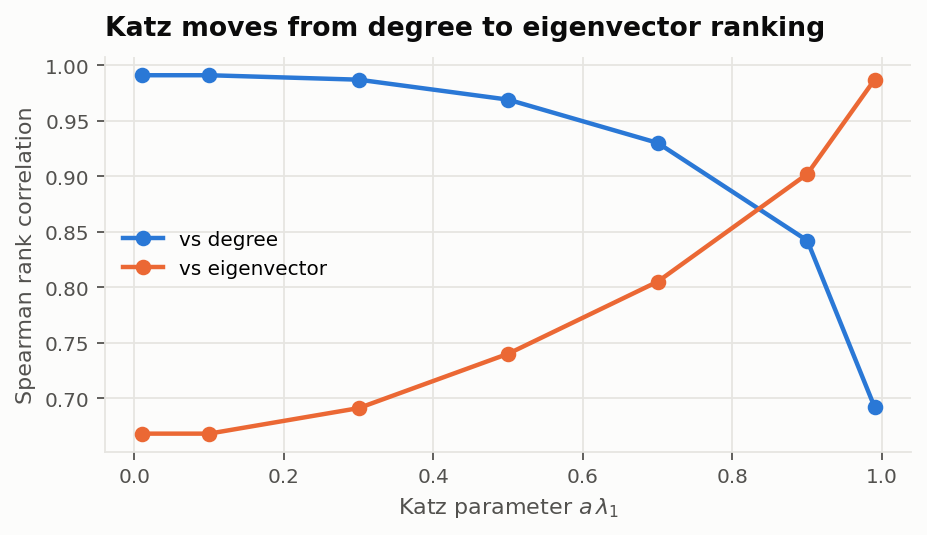
\includegraphics[width=0.85\linewidth]{katz_interpolation.png}
\caption{Spearman correlation of Katz with the degree and with the eigenvector, as the Katz parameter grows (largest component, 1,110 faculty).}
\label{fig:katz}
\end{figure}

\subsection{Communicability and the link between the campuses}
\textbf{Communicability} counts all the walks between two nodes, with shorter walks counting more,
$G = e^{A} = \sum_k A^k/k!$ (Estrada and Higham, 2010). Since $\lambda_1$ is well above $\lambda_2$ (12.5 and 9.9),
$e^{A}$ is also dominated by the leading eigenvector. So to compare groups we use the \textbf{communicability angle},
$\cos\theta_{pq} = G_{pq}/\sqrt{G_{pp}G_{qq}}$, which removes the size of each person's own walks (Estrada and Hatano,
2016). It is close to 1 when two people reach the network in the same way, and 0 when no walk joins them.

On the largest component, the mean $\cos\theta$ is 0.35 between two KGP faculty, 0.14 between two Roorkee faculty, and
only 0.066 between the campuses. The KGP value is high partly because its dense core holds many of the walks. But
the two campuses are clearly far apart in terms of walks too, not only in their 77 direct edges.

Who holds the campuses together? We define a \textbf{campus ratio}, the mean communicability between the campuses
divided by the geometric mean of the communicability within each campus. Then we remove each faculty member in turn
and recompute it. Removing Dr.~Pradip K.\ Maji (Roorkee) alone lowers it by 31\%. He has six co-authors at KGP, and he
is the bridge we met in the betweenness section. Next come Dr.~Narayan Chandra Das (26\%) and Dr.~Santanu
Chattopadhyay (22\%) from Rubber Technology at KGP, a field close to polymer engineering. Only 18 faculty lower the
ratio by more than 5\% (Fig.~\ref{fig:campus}). Betweenness finds only 5 of these top 10, so this measure gives a more
direct answer to who links the two IITs.

\begin{figure}[!t]
\centering
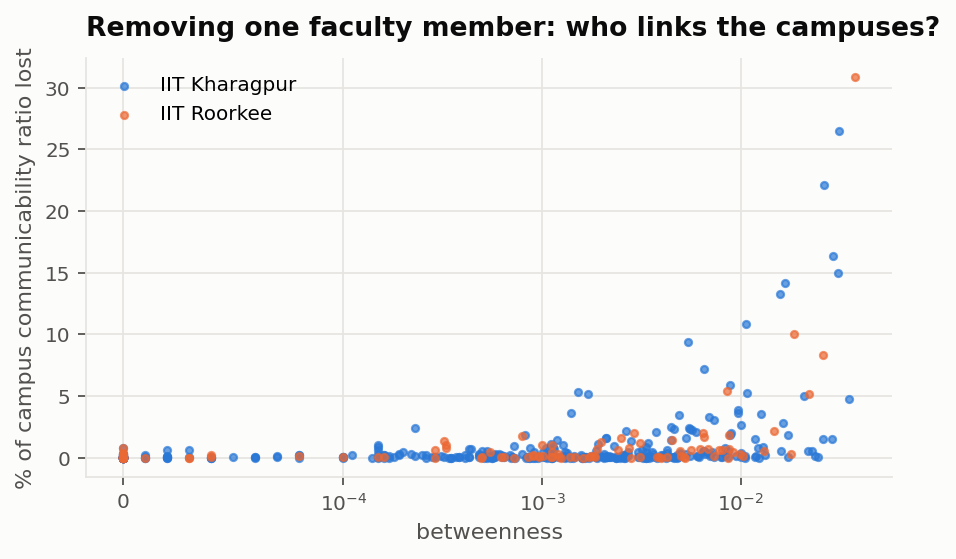
\includegraphics[width=0.85\linewidth]{cross_campus_removal.png}
\caption{Share of the campus ratio lost when one faculty member is removed, against their betweenness.}
\label{fig:campus}
\end{figure}

\subsection{Early connectors}
A static network forgets the order in which the ties appeared. In a \textbf{time-respecting walk}, each step must use a
tie from the same year or a later one. Grindrod, Parsons, Higham and Estrada (2011) count such walks with the product
$Q = \prod_t (I - aA_t)^{-1}$ over the yearly networks $A_t$. The row sums of $Q$, the \textit{broadcast} score, show
who can start chains that reach many people later.

We used one faculty network per year from 2016 to 2026, with $a = 0.5/\max_t \lambda_1(A_t)$. Over the 1,156 faculty
with at least one faculty co-author, the broadcast score mostly agrees with the degree ($\rho = 0.80$), as expected. But a few faculty rank much higher on broadcast than on
degree. Dr.~Amit Basak (KGP, Chemistry) is 11th on broadcast but 104th on degree, and Dr.~Sunando Dasgupta (KGP,
Chemical Engineering) is 12th against 157th. Both had faculty co-authors already in 2016, and these early ties lead,
through later ties, to many other people. So they were early connectors, a role that the final network hides.

\subsection{Katz and HITS on the citation network}
We also ran Katz and \textbf{HITS} on the citation network of Section~\ref{sec:cit}. HITS gives each paper an
\textit{authority} score (it is cited by good hubs) and a \textit{hub} score (it cites good authorities). The network
has 76 small groups of papers that cite each other, which happens when papers are written at the same time. The
largest has 10 papers by one author, and it sets the spectral radius to 2.93, so Katz must use $a < 1/2.93$. We use
$a = 0.17$.

HITS turns out to be unusable here. Its authority score is non-zero for only 5,086 of the 46,072 papers, and 72 of its
top 100 papers come from one metal-organic framework (MOF) chemistry group at KGP. This is the \textit{tightly knit
community} effect known for HITS (Lempel and Moran, 2000), where a small, densely linked group takes all the score.
Katz is much less affected (26 of its top 100), and it ranks papers almost like the in-degree ($\rho = 0.99$).

Can any of these scores predict the future? We computed each score on the network as it was at the end of 2020, and
compared it with the citations each paper got worldwide from 2021 to October 2026. We compare papers of the same year
only, so that age does not decide the result. In-degree, Katz and PageRank all reach a Spearman $\rho$ of 0.36 to 0.38,
while the worldwide citations up to 2020 reach 0.75 (Fig.~\ref{fig:pred}). In the 2020 network, HITS is non-zero for
only 30 papers, so it cannot rank them at all. This is expected, as our internal network is only a thin slice of all
citations.

The same test shows one more thing. Among papers with the same worldwide citations by 2020, those whose internal
citations were self-citations get slightly fewer citations later (partial $\rho = -0.087$). We checked this a second
way, inside groups of papers with the same year and similar past citations, and 15 of the 16 groups show the same sign.
Internal citations from other authors show no such effect ($+0.04$). So a self-citation does not signal later impact
the way an outside citation does. Since 88.5\% of the internal edges are self-citations, this is also why in-degree,
Katz and PageRank show the same small negative effect (partial $\rho$ about $-0.08$ for all three).

\begin{figure}[!t]
\centering
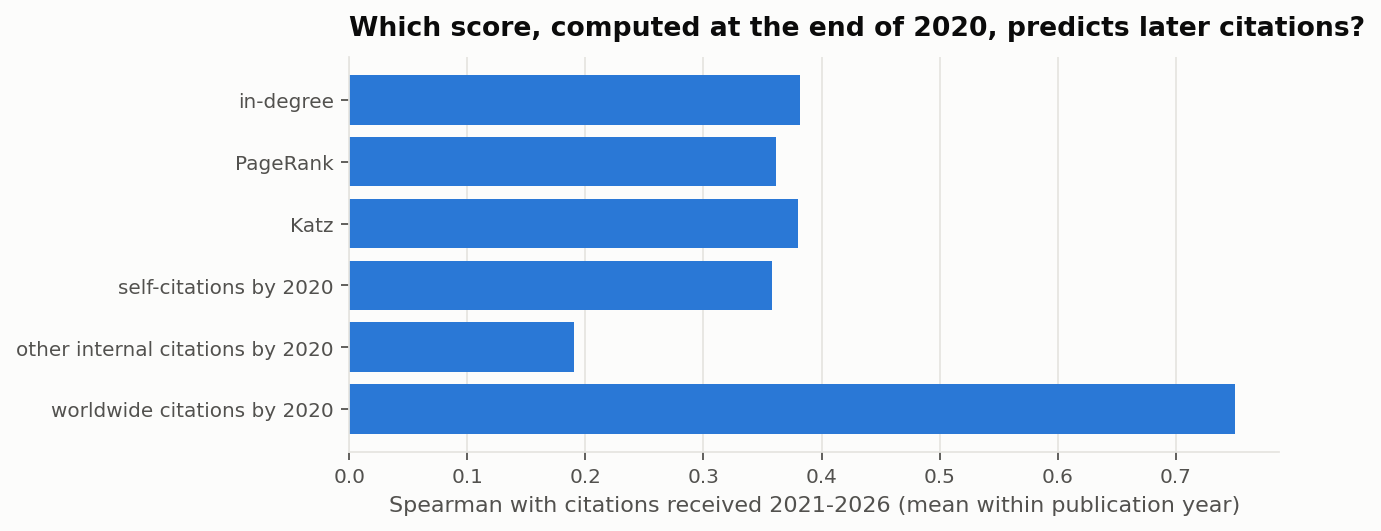
\includegraphics[width=\linewidth]{centrality_prediction.png}
\caption{Spearman correlation of each score at the end of 2020 with the citations received in 2021-2026, as a mean
over publication years (2016-2020 papers). HITS is left out, as it is non-zero for only 30 papers.}
\label{fig:pred}
\end{figure}

\subsection{Papers as groups}
In a co-authorship network, a paper with $k$ authors becomes $k(k-1)/2$ separate edges. A \textbf{hypergraph} keeps the
paper as one \textit{hyperedge} that holds all its authors. This matters for us because big teams make many pairs.
Our co-authorship data holds the 38,089 papers that have at least one linked faculty member and at most 50 authors,
with their full author lists. Of these, 696 have more than 10 authors. This is fewer than the 534 and 454 papers of
Section~\ref{sec:inst}, because those also count 259 papers with no linked faculty and 23 with more than 50 authors.
The 696 papers are 1.8\% of the 38,089, but they give 27\% of the author pairs, counted paper by paper.

We built the hypergraph of all 41,435 authors of these papers (faculty, students and outside co-authors), and computed the nonlinear
eigenvector centrality of Tudisco and Higham (2021). It scores authors and papers together,
\[
\lambda x = g\!\left(B f(y)\right), \qquad \mu y = \psi\!\left(B^{\top} \varphi(x)\right),
\]
where $B$ is the author-paper incidence matrix and $f, g, \varphi, \psi$ are fixed functions. We used their three
models. In the \textit{linear} model, a paper is worth the sum of its authors' scores, which is close to the eigenvector
of the pair network. In the \textit{max} model, a paper is worth about as much as its best author. In the
\textit{log-exp} model, a paper is worth the product of its authors' scores, which favours small teams.

All three models localise even more than the faculty eigenvector. The linear model puts 87\% of its weight on 10
authors and the max model 97\%, each on a different KGP lab. The log-exp model collapses onto only 33 authors, three of
them faculty, so it cannot rank faculty at all. The linear and max models agree only partly on faculty ($\rho = 0.69$).
The linear ranking is also fragile. Without the papers with more than 10 authors, 17 of its top 20 faculty change,
partly because two labs then almost tie for the top (their singular values differ by 0.3\%). A plain count of distinct
co-authors keeps 16 of its top 20 under the same change. About 10\% of authors have no OpenAlex ID and are kept by
name, which could join two people with the same name. Treating each of them as a new person on every paper changes
none of these results. So for our data, local measures like the number of co-authors are the safer way to rank faculty,
while global spectral measures mostly point to the densest lab.

\subsection{Do pairs become trios?}
A paper with three or more authors joins all of them at once, like a filled triangle (a \textit{simplex}). Benson and
others (2018) asked when three people who have each worked in pairs go on to write a paper as a trio, which they call
\textbf{simplicial closure}. We repeat their test. We take papers with at most 25 authors, as they did, use the papers
up to 2021 to see who has worked with whom, and check which trios write a joint paper from 2022 to 2026.

First, where do the triangles come from? In the pair network of all the authors of these papers, 96\% of the triangles exist only because
all three people are on one paper. In the faculty network the share is 54\%, partly because only 659 papers have three
or more faculty. So about half of the triangles behind the faculty clustering in Table~\ref{tab:null} come from such
papers, and the other half is real closure between separate pairs.

Second, the chance of a trio grows sharply with every pair that already exists (Fig.~\ref{fig:closure}). For three
people with no joint papers, it is about 3 in a billion. With one pair it is about 6 in a million, with two pairs 0.45\%,
and when all three pairs exist but never on one paper (an \textit{open triangle}) it is 3.7\%. Each extra pair raises
the chance by a factor of 8 to 2,000. The result is the same with a cap of 10 authors, and when the name-only authors
are split. Note that this is a chance per trio. There are far more trios with fewer pairs, so they still give most of
the new trios. Of all new trios, 20\% had no earlier pair, 49\% had one and 30\% had two, and only 0.8\% closed an
open triangle. So 80\% of new trios follow at least one earlier pair.

Third, which open triangles will close? We ranked them by simple scores, like the harmonic mean of the three tie
strengths, and checked how well this finds the 147 that closed. The best score is only 1.3 times better than random
(ROC AUC 0.56, $p = 0.005$), and it is not significant with the 10-author cap. So a trio is far more likely once all its
pairs exist, but which trio actually forms is hard to predict from the network alone.

\begin{figure}[!t]
\centering
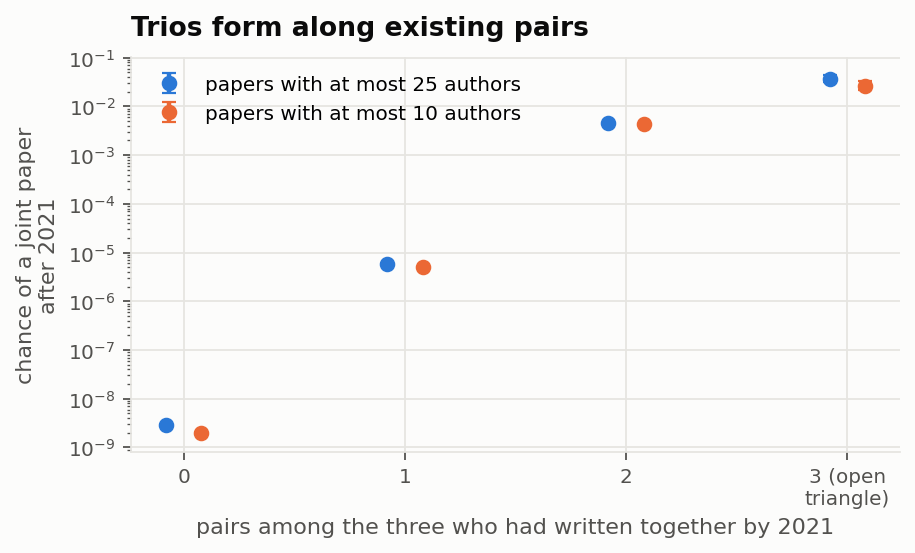
\includegraphics[width=0.85\linewidth]{simplicial_closure.png}
\caption{Chance that three authors write a joint paper in 2022-2026, by how many pairs among them had written together
by 2021 (log scale). Error bars are 95\% intervals, and most are smaller than the dots.}
\label{fig:closure}
\end{figure}

\subsection{Do faculty cite their co-authors?}\label{sec:coauthcite}
Up to now, we have studied the citation network and the co-authorship network one at a time. But they are two layers
on the same people, so we can ask how the two layers are linked. Wallace, Larivi\`ere and Gingras (2012) and Martin,
Ball, Karrer and Newman (2013) found that scientists cite their co-authors much more often than other people. We test
this on our 1,410 faculty.

We say that faculty member A cites B when A is an author of a citing paper and B is an author of the cited paper. As
we saw in Section~\ref{sec:cit}, most internal citations are self-citations, and a self-citation between two co-authors
would make this test trivial. So we use a \textit{strict} rule here. The citing paper and the cited paper must have no
author in common at all. This leaves 10,205 of the 50,372 faculty-to-faculty citations, between 4,999 ordered pairs of
faculty.

For each ordered pair, we take the distance between A and B in the faculty co-authorship network, and we find the share
of pairs at each distance where A cites B (Table~\ref{tab:coauthcite}). Co-authors often share a department, a topic
and a high output, and each of these raises the chance of a citation on its own. So we compare each group with the
pairs that are four or more steps apart and are of the same kind (the same department, institute or campus relation,
the same main subfield and a similar number of papers). The ratio of observed to expected citing pairs (O/E) then
shows the extra effect of the co-author tie.

Co-authors cite each other in 14.0\% of the pairs, against 0.11\% for pairs four or more steps apart, and the O/E is
10.3. The effect falls with distance, to 7.1 at two steps and 3.4 at three steps. It is strongest when the tie crosses
a boundary (Fig.~\ref{fig:coauthcite}). Co-authors from two departments of the same IIT cite each other 30 times as
often as similar faculty far apart, and co-authors from the two IITs 29 times as often. Inside a department the ratio is
7.2, because faculty of one department cite each other often anyway.

\begin{table}[!t]
\centering
\caption{Share of faculty pairs in which A cites B, by distance in the co-authorship network (strict rule). In brackets,
the O/E against pairs of the same kind that are four or more steps apart.}
\label{tab:coauthcite}
\footnotesize
\setlength{\tabcolsep}{3pt}
\begin{tabular}{@{}lrrr@{}}
\toprule
\textbf{Distance} & \textbf{Same dept.} & \textbf{Other dept.} & \textbf{Other IIT} \\
\midrule
\inputrows{tables/coauthor_distance.tex}
\end{tabular}
\end{table}

\begin{figure}[!t]
\centering
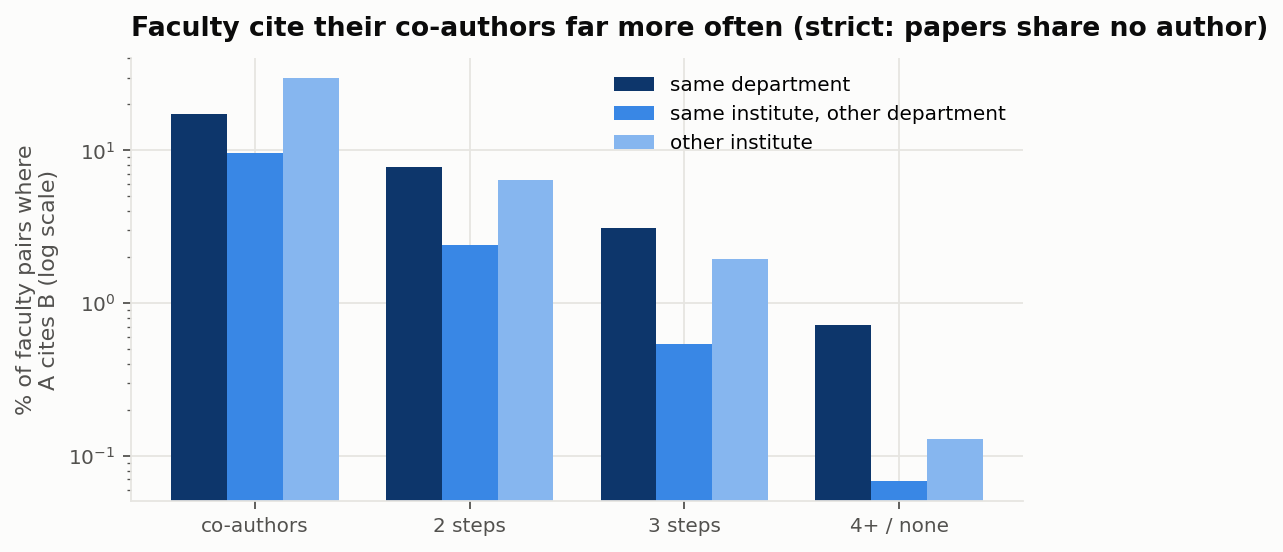
\includegraphics[width=\linewidth]{coauthor_citation_distance.png}
\caption{Share of faculty pairs in which A cites B, by co-authorship distance (log scale, strict rule).}
\label{fig:coauthcite}
\end{figure}

Does citing come before working together, or after it? We split the time at the end of 2020 and use the 928 faculty
who published both before and after. Among the pairs that had not written together by 2020, the pairs where one had
cited the other started a joint paper in 2021-2026 in 7.0\% of cases, against 0.24\% for the other pairs. That is 3.6
times what pairs of the same kind show. The other direction is just as strong. Among the pairs with no citation by
2020, co-authors started to cite each other in 20\% of cases, which is 3.9 times the expected value. So each layer
predicts the next step in the other layer. For the 383 pairs whose first contact came after 2018 and who later both
wrote together and cited each other, the joint paper came first in 56\% of cases and the citation in 31\%. Our data
starts in 2016, so we only describe this split and do not test it.

As we know from our lectures, \textbf{reciprocity} is the share of directed links that also go back. 23\% of the citing
pairs cite each other in both directions, against 2.2\% in a configuration model with the same in-degrees and
out-degrees (2.5\% in 10 rewired networks). It is 44\% for co-authors and still 20\% for pairs who never wrote together.

Last, we measure \textbf{inwardness} (Baccini, De Nicolao and Petrovich, 2019), which is the share of an institute's
citations that come from its own papers. We report it only for whole institutes. In our set it is 10.2\% at KGP and
10.4\% at Roorkee. Almost all of it is self-citation. Without the citations where the two papers share an author, it
is 0.7\% at KGP and 1.0\% at Roorkee. The total rises for recent papers, to 14\% and 16\% for the papers of 2025, but
only the self-citation part rises. A young paper gets its first citations mostly from its own authors, so this is an
effect of age and not a trend. Both values are lower bounds, because our set holds only the verified science and
engineering papers of each IIT.

\subsection{Core and periphery of the citation network}\label{sec:bowtie}
A citation network of papers has almost no cycles, because papers cite older papers. So its strongly connected groups
are tiny, at most 10 papers in our data. When we join all the papers of one faculty member into one node, cycles
appear, because A can cite B in one year and B can cite A later. As we know from our lectures, a \textbf{strongly
connected component} is a set of nodes in which every node can reach every other node along directed links. Broder and
others (2000) described a directed network as a \textbf{bow-tie} around its largest strongly connected component, the
\textit{core}. The \textit{IN} part holds the nodes that can reach the core but cannot be reached from it, the
\textit{OUT} part holds the reverse, and \textit{tendrils} hang off IN or OUT. Tim\'ar, Goltsev, Dorogovtsev and Mendes
(2017) studied this structure in more detail.

Our faculty network has a link from A to B when A cites B, where A is not an author of the cited paper and B is not an
author of the citing paper. It has 6,626 citing pairs. In this network, IN holds faculty who draw on the core, and OUT
holds faculty the core draws on. 741 of the 1,110 faculty with at least one citation link form one core, with 406
from KGP and 335 from Roorkee (Table~\ref{tab:bowtie}). 612 of the 741 core members cite, or are cited by, a core member
of the other IIT, so the core spans both campuses. This is very different from the co-authorship network, where the
campuses share only 77 links. 1,828 of the 6,626 citing pairs (28\%) join the two IITs, so citations cross the campuses
much more easily than collaboration does.

\begin{table}[!t]
\centering
\caption{Bow-tie parts of the faculty citation network}
\label{tab:bowtie}
\footnotesize
\begin{tabular}{@{}lrrr@{}}
\toprule
\textbf{Part} & \textbf{KGP} & \textbf{Roorkee} & \textbf{Total} \\
\midrule
\inputrows{tables/bowtie.tex}
\end{tabular}
\end{table}

Is this core special? We rewired the network 10 times, keeping the number of citations each faculty member makes and
receives. The random networks give a core of 761 faculty (753 to 767), about the same as the real 741. So the size of
the core follows from the citation counts alone. What the bow-tie does show is who sits where. Core members have a
median of 39 papers and an h-index of 12, against 13 papers and 4 for IN and 13 papers and 6 for OUT. The 300 faculty
with no citation link to another faculty member have a median of only 3 papers. The core grew from 19 faculty, for the
citations made up to 2018, to 741 by 2026 (Fig.~\ref{fig:bowtie}). With the strict rule of
Section~\ref{sec:coauthcite}, the core has 622 faculty and the random networks give 651, so the result is the same.

\begin{figure}[!t]
\centering
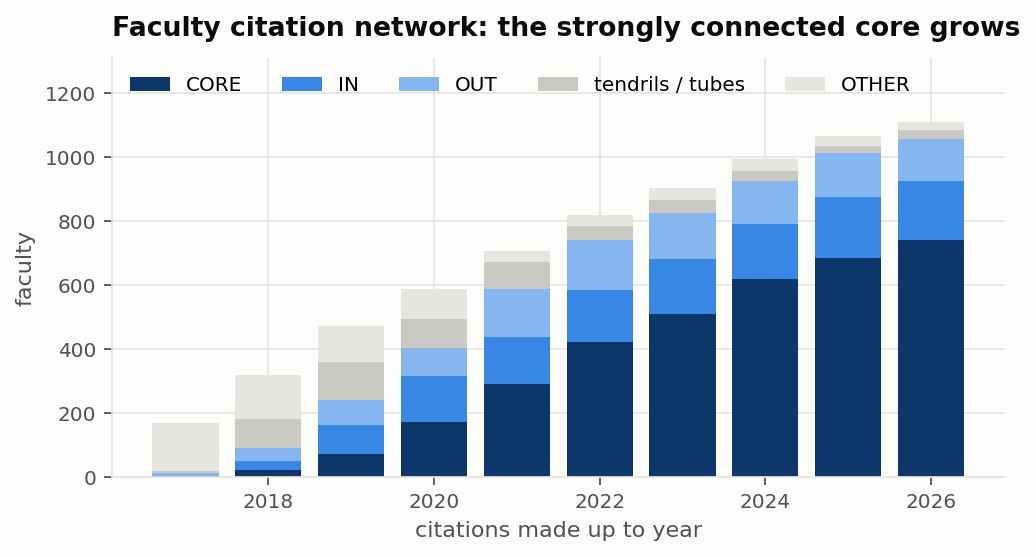
\includegraphics[width=\linewidth]{bowtie_growth.png}
\caption{Bow-tie parts of the faculty citation network, for the citations made up to each year.}
\label{fig:bowtie}
\end{figure}

We also placed the 48 departments with at least 5 faculty on one line, using the 9,578 citations between departments.
\textbf{SpringRank} (De Bacco, Larremore and Moore, 2018) finds positions such that, for most citations, the cited
department sits above the citing one. It agrees with a simple net balance (citations received minus citations made,
divided by their sum) at $\rho = 0.94$. Among the larger departments, KGP Electrical Engineering, Electronics and
Electrical Communication Engineering and Mechanical Engineering are near the top. KGP Electrical Engineering, for
example, is cited 244 times by other departments and cites them 69 times. Roorkee Hydrology (cited 170 times, cites 341
times), Water Resources Development and Management (248 and 381) and Architecture and Planning are near the bottom. They
draw more on other departments than other departments draw on them. This is a position in the citation flow between
our two IITs, and not a measure of quality.

\subsection{Do mixed-department teams get more citations?}
Work that joins several fields is often said to have more impact, but studies disagree, and the answer depends on how
the mix is measured (Wang, Thijs and Gl\"anzel, 2015). Since we know the department of every faculty member, we can test
one simple form of it, which is a team that mixes departments. We take the 7,954 papers with at least two of our
faculty. Of these, 4,689 have all their faculty in one department, 3,130 mix departments of the same IIT and 135 mix the
two IITs. A recount of the mixed papers from \texttt{group3\_data.csv} gives the same 3,265.

Raw citations depend on the field and the age of a paper, so we use the \textbf{field-weighted citation impact}
(FWCI) from OpenAlex. It is the citations of a paper divided by the world average for papers of the same field, year
and type, so 1 is the world average. We use the papers up to 2023, since newer papers have had little time to be cited.
Bigger teams get more citations and also mix departments more often, so we hold the team size fixed in three ways.
\begin{enumerate}
\item We compare mixed and one-department papers only inside groups with the same number of faculty, the same number of
authors, the same year and the same field. The mean of $\log(1 + \mathrm{FWCI})$ differs by only 0.006.
\item In a regression on the same controls, the effect of mixing departments is $-0.001$ (95\% interval $-0.036$ to
$0.033$, $p = 0.94$). The chance of being in the world's top 10\% changes by $+0.1$ points ($p = 0.90$).
\item For the 450 faculty members who have both kinds of papers, we compare each person with themselves. Their mixed
papers do better for 54\% of them, and the difference is not significant (Wilcoxon $p = 0.82$).
\end{enumerate}
How far apart the departments are does not matter either. We measured it with the Rao-Stirling diversity (Stirling,
2007), using the distance between the departments' subfield profiles, and found no effect ($p = 0.26$). So in our data,
mixing departments brings no citation gain once the team size is fixed. Papers that join the two IITs do slightly worse
($-0.12$ in the matched groups and $-0.11$ in the regression, $p = 0.025$), but there are only 99 such papers, and with
all years included the effect is not significant ($p = 0.07$). We call this a weak result.

\subsection{Department strengths and where they move next}
We describe what a department is strong in with the \textbf{revealed comparative advantage} of each OpenAlex subfield,
$\mathrm{RCA}_{ds} = (X_{ds}/X_d)/(X_s/X)$, where $X_{ds}$ is the number of papers of department $d$ in subfield $s$
(Hidalgo, Klinger, Barab\'asi and Hausmann, 2007). An RCA above 1 means the department puts a larger share of its papers
into that subfield than our two IITs do overall. We call a department strong in a subfield when its RCA is at least 1
and it has at least 5 papers there, so that one or two papers do not count as a strength. We use the 46 departments
with at least 5 faculty and 100 papers. The full lists are in \texttt{dept\_area\_strengths.csv}, and some departments
changed a lot between 2016-2020 and 2021-2026. For example, KGP Architecture and Regional Planning went from 1 to 50
papers in Building and Construction, KGP Mathematics from 3 to 52 in Algebra and Number Theory, and KGP Electronics and
Electrical Communication Engineering from 8 to 77 in Electronic, Optical and Magnetic Materials.

Can we predict which subfields a department moves into? Hidalgo and others (2007) showed that countries start to export
products that are related to what they already export, and Guevara and others (2016) found the same for research
fields. Two subfields are related when the same faculty are strong in both. We measure this with the 742 faculty who had
at least 5 papers in 2016-2020. The \textbf{density} of a subfield for a department is then the share of its related
subfields where the department was already strong in 2016-2020, with closer subfields counting more.

Of the 5,203 department-subfield pairs that were not a strength in 2016-2020, 204 became one in 2021-2026. The density
ranks them with a ROC AUC of 0.83, where 0.5 would be a random guess. In the most related fifth of the pairs, 17\%
became a strength, against 0.5\% for the 2,053 pairs with no related strength at all (Fig.~\ref{fig:deptareas}). When we shuffle the subfield
labels, the AUC drops to 0.51 (95\% range 0.46 to 0.56), and none of 500 shuffles reaches 0.83. For the 4,416 pairs with
no paper at all before 2021, of which 56 became a strength, the AUC is still 0.83. A department's own RCA in 2016-2020
also predicts well (0.82), so we also fitted both, leaving out one department at a time. Density alone gives 0.82, RCA
alone 0.77 and the two together 0.89. So relatedness adds information that the department's own past does not hold.

\begin{figure}[!t]
\centering
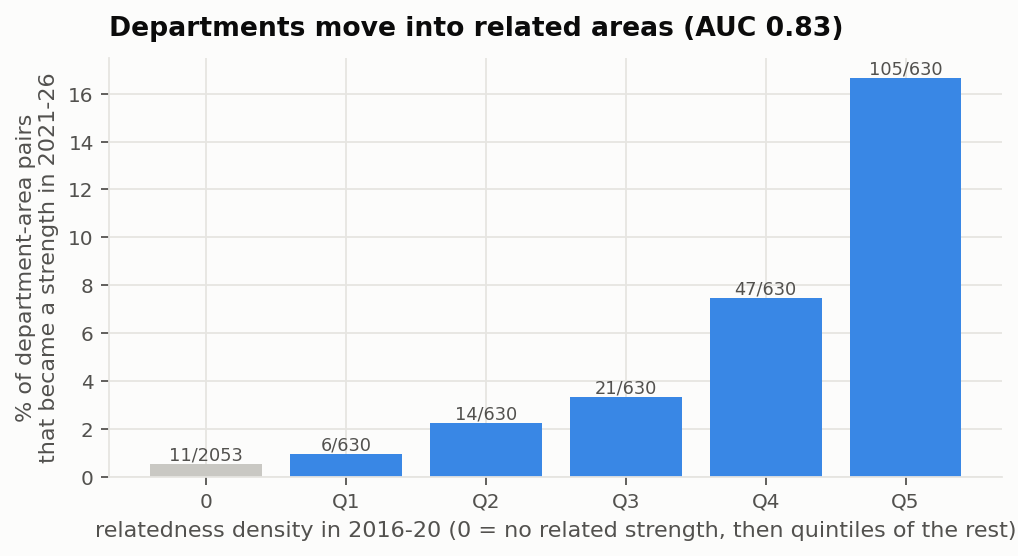
\includegraphics[width=0.9\linewidth]{dept_area_prediction.png}
\caption{Share of department-subfield pairs that became a strength in 2021-2026, by their relatedness density in
2016-2020. The first bar holds the pairs with no related strength at all, and the others are fifths of the rest. The
labels give new strengths over pairs.}
\label{fig:deptareas}
\end{figure}

Last, we ran the \textbf{fitness-complexity} map of Tacchella and others (2012). It is a nonlinear centrality on the
department-subfield matrix that gives a department a high fitness when it is strong in many subfields, and especially in
subfields that few other departments are strong in. The values of most departments shrink towards zero as the map runs,
which is known to happen when the matrix is not perfectly nested (Pugliese, Zaccaria and Pietronero, 2016). The ranking
itself is stable ($\rho = 0.9998$ between 50 and 100 steps). The top departments are KGP Agricultural and Food
Engineering, Roorkee Biosciences and Bioengineering, and the Mathematics departments of both IITs.

%===========================================================
\section{Connections with Other Indian Institutes}\label{sec:india}
%===========================================================
The faculty network only covers the two IITs. As a last step, we look at their co-authorship with all other Indian
institutes.

\subsection{Partner institutes}
We count the shared papers between each IIT and each Indian partner. KGP works most with IISc Bangalore (340 papers),
IIT Bombay (317) and Jadavpur University (305), while Roorkee works most with IIT Delhi (310), the National Institute of
Hydrology (266) and IIT Kharagpur (231) (Fig.~\ref{fig:partners}). These lists make sense in terms of both location and
field. The KGP list has several institutes from Kolkata, like Jadavpur University, and the National Institute of
Hydrology is based in Roorkee itself, which fits Roorkee's strength in water research.

\begin{figure}[!t]
\centering
\includegraphics[width=0.95\linewidth]{top_partners.png}
\caption{Top 12 Indian partner institutes of each IIT, by co-authored papers.}
\label{fig:partners}
\end{figure}

\subsection{Similar or complementary research}
Do the IITs work with institutes doing the same research, or with ones that fill a gap? To measure this, we take the
top 20 research subfields of the IIT and of the partner, and compute their \textbf{Jaccard similarity},
\[
J(A, B) = \frac{|A \cap B|}{|A \cup B|}
\]
which is 1 if the two lists are identical, and 0 if they have nothing in common.

For the top 25 partners of each IIT, the median is 0.60, so most partners do similar research. A few strong partners
are complementary though, like the Indian Statistical Institute (0.18, KGP), and the National Institute of Hydrology
and the Indian Institute of Remote Sensing (0.21 each, Roorkee). These are specialised institutes, so the collaboration
is probably focused on one topic, such as statistics, hydrology or remote sensing.

%===========================================================
\section{Dashboard and Conclusions}
%===========================================================
All of these results are also available on an
\href{https://avi1o1.github.io/DPCN_A2_ResearchMapper/}{interactive website}, with a switch for KGP, Roorkee or both. Clicking on
a faculty member lists all their papers in our dataset, so anyone can check a person's numbers for themselves.

To conclude, both IITs almost doubled their science and engineering output over ten years, and about two thirds of
their ranked journal papers are in Q1. Their faculty h-index is about half of a career h-index, since we only count ten
years of papers, and it grows by about one point every year. Environmental Science is high because a lot of water and
climate engineering is filed under it. Papers with more than 10 authors make up only 2\% of the output, but 6 of KGP's
ten most cited papers, and removing them leaves the typical numbers unchanged, moving only the top. Citations are
heavy-tailed (closer to lognormal than a clean power law), and new citations go preferentially to papers that are
already cited. Most citations within an institute are self-citations, so we also rank papers without them, and correct
PageRank for age. Since 2023, Indian research has been citing the IITs more than they cite it. Faculty work in tight,
hierarchical groups within each campus, forming a small world that has grown denser every year. This network survives
the random loss of faculty, but losing about 100 bridging faculty would split the two campuses apart, and ideas spread
best from its core. Faculty cite their co-authors far more often than other faculty, and citing and writing together
each lead to the other. Teams that mix departments get no citation gain, but departments do move into research areas
close to what they already do. Every step of this work is a script in our repository, so anyone can repeat it.

The second part of our work adds two lessons. First, the high-quality output of both IITs, whether Q1 or IF $>$ 10,
comes mostly from teams of fewer than 10 authors (92\% of the IF $>$ 10 papers). Second, matrix functions and hypergraphs show the
collaboration network as a set of separate dense labs. Measures that use the whole network at once pick out one of
these labs, while local measures stay stable. A new trio also becomes far more likely with every earlier pair among
its members, and 80\% of new trios follow at least one such pair.

\end{document}
